\documentclass[12pt]{article}
\usepackage[margin=1in]{geometry}
\usepackage{amsthm, amsmath, amsfonts, amssymb}
\usepackage{graphicx}
\usepackage[shortlabels]{enumitem}
\usepackage{setspace}
\usepackage{tcolorbox}
\usepackage[
  lambda,
  advantage,
  operators,
  adversary,
  landau,
  probability,
  sets,
  % notions,
  % logic,
  % ff,
  % mm,
  % primitives,
  % oracles,
  events,
  % complexity,
  asymptotics,
  keys,
]{cryptocode}
\doublespacing
\usepackage{hyperref}

\usepackage{pgfplots}
\pgfplotsset{compat=1.18}

\definecolor{cblueA}{HTML}{185FA5}
\definecolor{cblueB}{HTML}{378ADD}
\definecolor{cred}{HTML}{A32D2D}
\definecolor{ccoral}{HTML}{D85A30}
\definecolor{camber}{HTML}{BA7517}

%%% cryptocode tweaks
% Multi-letter variables, e.g., "ctr"
\NewDocumentCommand\var{m}{\ensuremath{\mathit{#1}}}
% Make keys and polynomials look like other identifiers.
% (No idea why cryptocode treats them specially.)
\RenewDocumentCommand\pckeystyle{m}{\ensuremath{\var{#1}}}
\RenewDocumentCommand\pcpolynomialstyle{m}{\ensuremath{\var{#1}}}
% Add 1pt padding to \gamechange (based on original definition).
\renewcommand{\gamechange}[2][gamechangecolor]{%
  {\setlength{\fboxsep}{1pt}%
    \colorbox{#1}{#2}}}
% Shorthand for \pcalgostyle
\NewDocumentCommand\algo{}{\pcalgostyle}
% Oracles
\NewDocumentCommand{\mathsc}{m}{{\normalfont\textsc{#1}}}
\RenewDocumentCommand\pcoraclestyle{m}{\ensuremath{\mathsc{#1}}}
\NewDocumentCommand\oracle{m}{\pcoraclestyle{#1}}
% Games
\newcommandx{\game}[4][3=\adv,4=(\secpar)]{{\operatorname{#1}_{#2}^{#3}#4}}
%\newcommand{\Game}{\algo{Game}}
% Misc
\newcommand{\pcsc}{\,;~}

\newcommand{\N}[0]{\mathbb{N}}
\newcommand{\Z}[0]{\mathbb{Z}}
\newcommand{\Q}[0]{\mathbb{Q}}
\newcommand{\F}[0]{\mathbb{F}}
\newcommand{\G}[0]{\mathbb{G}}
\newcommand{\pr}[1]{\text{Pr}\left[#1\right]}
\newcommand{\overarrow}[1]{\stackrel{#1}{\rightarrow}}
\newcommand{\verts}[1]{\left\vert #1\right\vert}
\newcommand{\M}{\mathcal{M}}
\newcommand{\C}{\mathcal{C}}
\newcommand{\K}{\mathcal{K}}
\newcommand{\Kpriv}{\mathcal{K}_{\text{priv}}}
\newcommand{\Kpub}{\mathcal{K}_{\text{pub}}}

\newtheorem{claim}{Claim}
\newtheorem{conj}{Conjecture}
\newtheorem{question}{Question}
\newtheorem{exercise}{Exercise}
\newtheorem{reading}{Reading}
\newtheorem{thm}[claim]{Theorem}
\newtheorem{lemma}[claim]{Lemma}
\newtheorem{prop}[claim]{Proposition}
\newtheorem{cor}[claim]{Corollary}
\theoremstyle{definition}
\newtheorem{definition}{Definition}

\theoremstyle{remark}
\newtheorem*{rem}{Remark}

\theoremstyle{definition}
\newtheorem{example}{Example}[section]


\begin{document}

\begin{exercise}

\end{exercise}
\begin{exercise}

\end{exercise}
\begin{exercise}

\end{exercise}
\begin{exercise}
Let $(G, S, V)$ be a secure signature scheme with the message space $\{0,1\}^\lambda$. Let $\hat{G}$ be a new key generation function that simply calls $G$ twice and returns a pair of secret keys, $(sk_0, sk_1)$, and the corresponding pair of public keys, $(pk_0, pk_1)$. Which of the following signature schemes, $(\hat{G}, \hat{S}, \hat{V})$, are secure? Show an attack or prove security (by reduction).
\begin{enumerate}[(a)]
\item Prove that ``Sign halves'' is \textbf{not} secure: $$\hat{S}((sk_0, sk_1), (m_L, m_R)) = (S(sk_0, m_L), S(sk_1, m_R)),$$ $$\hat{V}((pk_0, pk_1), (m_L, m_R), (\sigma_0, \sigma_1)) = V(pk_0, m_L, \sigma_0)\wedge V(pk_1, m_R, \sigma_1).$$
The attack game below shows how the attacker $\adv$ can forge a signature for the "sign halves" signature scheme.
\begin{figure}[tbhp]
\centering
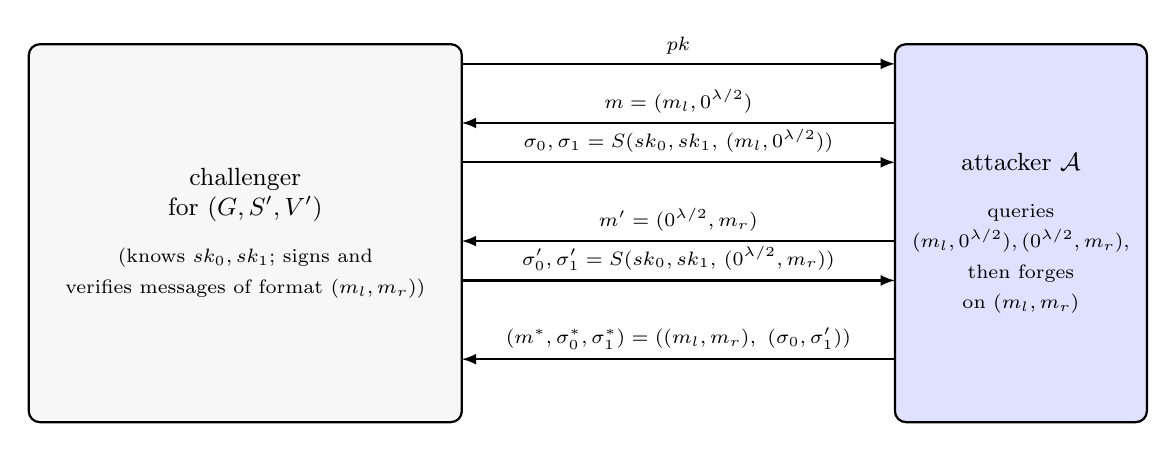
\begin{tikzpicture}[font=\small, >=latex,
   wire/.style={->, thick}]

% ---- Challenger (modified, insecure scheme) ----
\draw[thick, rounded corners, fill=black!3] (0,-0.3) rectangle (5.5,4.5);
\node[align=center] at (2.75,2.1)
  { challenger\\ for $(G,S',V')$\\[6pt] \scriptsize(knows $sk_0, sk_1$; signs and\\ \scriptsize verifies messages of format $(m_l, m_r)$)};

% ---- Attacker ----
\draw[thick, rounded corners, fill=blue!12] (11,-0.3) rectangle (14.2,4.5);
\node[align=center] at (12.6,2.1) {attacker $\adv$\\[6pt] \scriptsize queries \\ \scriptsize $(m_l,0^{\lambda/2}), (0^{\lambda/2}, m_r)$,\\ \scriptsize then forges\\ \scriptsize on $(m_l, m_r)$};

% ---- pk wire (challenger -> attacker) ----
\draw[wire] (5.5,4.25) -- (11,4.25);
\node[font=\scriptsize, above] at (8.25,4.25) {$pk$};

% ---- query (attacker -> challenger) ---- 
\draw[wire] (11,3.5) -- (5.5,3.5); 
\node[font=\scriptsize, above] at (8.25,3.5) {$m = (m_l,0^{\lambda/2})$};

% ---- response (challenger -> attacker) ----
\draw[wire] (5.5,3) -- (11,3);
\node[font=\scriptsize, above] at (8.25,3) {$\sigma_0, \sigma_1 = S({sk}_0, {sk}_1,\,(m_l,0^{\lambda/2}))$};

% ---- query (attacker -> challenger) ----  
\draw[wire] (11,2) -- (5.5,2); 
\node[font=\scriptsize, above] at (8.25,2) {$m' = (0^{\lambda/2}, m_r)$};

\draw[wire] (5.5,1.5) -- (11,1.5);
\node[font=\scriptsize, above] at (8.25,1.5) {$\sigma'_0, \sigma'_1 = S({sk}_0, {sk}_1,\, (0^{\lambda/2}, m_r))$};

% ---- forgery (attacker -> challenger) ----
\draw[wire] (11,0.5) -- (5.5,0.5);
\node[font=\scriptsize, above] at (8.25,0.5) {$(m^*,\sigma_0^*, \sigma_1 ^*) = ((m_l, m_r),\ (\sigma_0, \sigma_1'))$};

\end{tikzpicture}
\end{figure}
Let's discuss the correctness of the attack. First let's dive into the freshness of the message. The oracle has only seen the messages $(m_l, 0^{\lambda/2})$ and $(0^{\lambda/2}, m_r)$ and has never been queried for $(m_l, m_r)$ together hence this query does not already exist in its set, being fresh and acceptable.
For the case of the signatures being verified, we can check the process. We know that the verification algorithm is $V(pk_0, m_L, \sigma_0)\wedge V(pk_1, m_R, \sigma_1)$. Since both $sigma'_1$ and $sigma_0$ have been queried from the oracle they are valid messages for $m_r$ and $m_l$ correspondingly, which means that the verifier will pass.
\item Show that ``Sign with randomness'' is \textbf{not} secure: $$\hat{S}(sk_0, m) = [\text{choose random }r\in\{0,1\}^\lambda; \text{output }(r, S(sk_0, m\oplus r), S(sk_0, r))],$$ $$\hat{V}(pk_0, m, (r, \sigma_0, \sigma_1)) = V(pk_0, m\oplus r, \sigma_0)\wedge V(pk_0, r, \sigma_1).$$
\begin{figure}[tbhp]
\centering
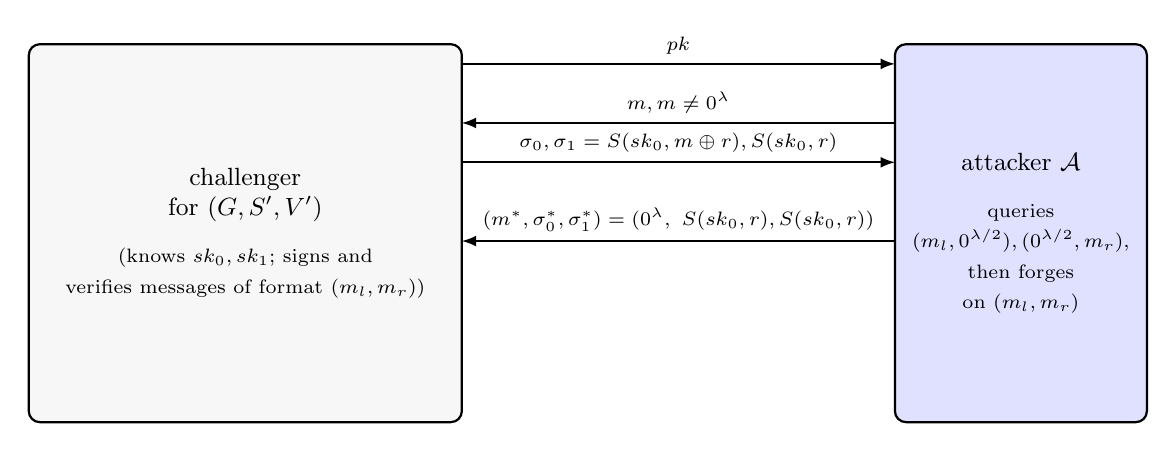
\begin{tikzpicture}[font=\small, >=latex,
   wire/.style={->, thick}]

% ---- Challenger (modified, insecure scheme) ----
\draw[thick, rounded corners, fill=black!3] (0,-0.3) rectangle (5.5,4.5);
\node[align=center] at (2.75,2.1)
  { challenger\\ for $(G,S',V')$\\[6pt] \scriptsize(knows $sk_0, sk_1$; signs and\\ \scriptsize verifies messages of format $(m_l, m_r)$)};

% ---- Attacker ----
\draw[thick, rounded corners, fill=blue!12] (11,-0.3) rectangle (14.2,4.5);
\node[align=center] at (12.6,2.1) {attacker $\adv$\\[6pt] \scriptsize queries \\ \scriptsize $(m_l,0^{\lambda/2}), (0^{\lambda/2}, m_r)$,\\ \scriptsize then forges\\ \scriptsize on $(m_l, m_r)$};

% ---- pk wire (challenger -> attacker) ----
\draw[wire] (5.5,4.25) -- (11,4.25);
\node[font=\scriptsize, above] at (8.25,4.25) {$pk$};

% ---- query (attacker -> challenger) ---- 
\draw[wire] (11,3.5) -- (5.5,3.5); 
\node[font=\scriptsize, above] at (8.25,3.5) {$m , m \neq 0 ^ \lambda$};

% ---- response (challenger -> attacker) ----
\draw[wire] (5.5,3) -- (11,3);
\node[font=\scriptsize, above] at (8.25,3) {$\sigma_0, \sigma_1 = S({sk}_0,m \oplus r), S({sk}_0, r)$};

% ---- forgery (attacker -> challenger) ----
\draw[wire] (11,2) -- (5.5,2);
\node[font=\scriptsize, above] at (8.25,2) {$(m^*,\sigma_0^*, \sigma_1 ^*) = (0^\lambda,\ S({sk}_0, r), S({sk}_0, r))$};
\end{tikzpicture}
\end{figure}
Since the oracle has never been queried for the message zero, this message is fresh and is accepted. Regarding the verification, the random signature is valid if we put the message as zero for $\sigma_0 ^*$ since $$0^\lambda \oplus r = r$$. 
\item Prove that ``Accept one valid'' is secure: $$\hat{S}((sk_0, sk_1), m) = (S(sk_0, m), S(sk_1, m)),$$ $$\hat{V}((pk_0, pk_1), m, (\sigma_0, \sigma_1)) = V(pk_0, m, \sigma_0)\vee V(pk_1, m, \sigma_1).$$ (Hint: Consider using that $\pr{\sigma_0\text{ or }\sigma_1\text{ is valid}} \leq \pr{\sigma_0\text{ valid}} + \pr{\sigma_1\text{ valid}}$ from Exercise 4 of last week).
\end{enumerate}
\end{exercise}

\end{document}